%!TEX root = ../report.tex
\chapter{Experiments}
\label{experiments}
In this chapter the experimental results are outlined. The experimental method is outlined in chapter~\ref{method}. For the experiment, a number of simulation runs are recorded in USAR Sim. The map is then 

\section{Experimental Runs}
\subsection{Map 1: IranOpen 2012 - Pre 2}
This map was used in the Iran Open 2012 competition \cite{iran2012}. The map features a grey hospital-like environment with grey tiled floors and walls. In figure~\ref{fig:map1} a screenshot of the environment is shown along with the map after the Weighted Scan Matcher was run on the simulation data. 

\begin{figure}[ht]
\centering
\subfigure[Screenshot]{
	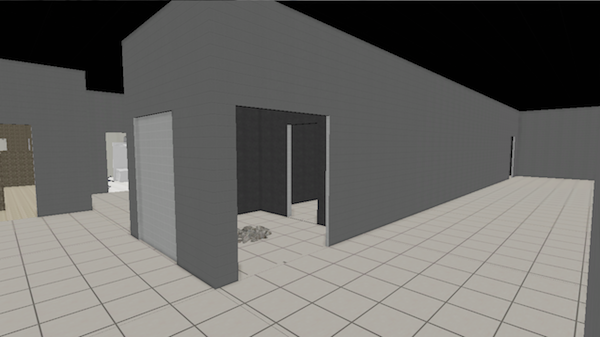
\includegraphics[width=0.5\textwidth]{images/experiment/map1/screenshot.png}
	\label{fig:map1-screenshot}
}
\subfigure[Map created with the WSM]{
	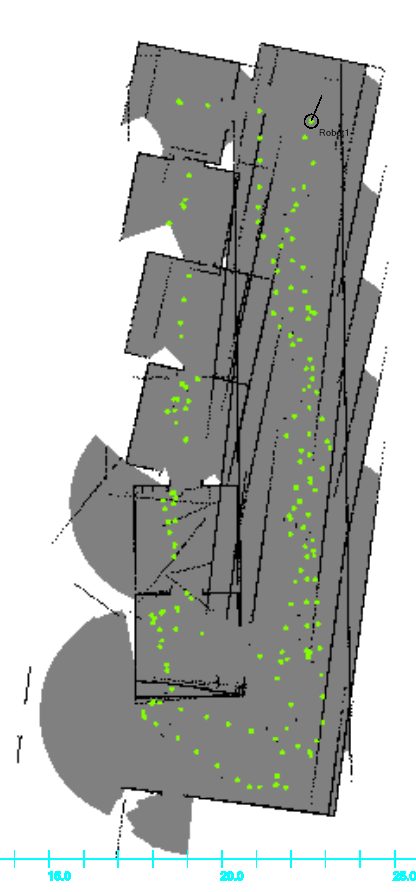
\includegraphics[width=0.3\textwidth]{images/experiment/map1/slam.png}
	\label{fig:map1-map}
}
  \caption{The ground truth, inertia sensor and slam path of the robot on a piece of map 1.}
  \label{fig:map1}
\end{figure}

The map shows a lot of noise and errors. As can be seen in figure~\ref{fig:apx:map1-paths} (in the appendix), the inertia sensor gives a rather good location-estimate, but the rotation estimate from position 160 onwards is off by more than $10\degree$. The scanmatcher fails regularly because it takes the inertia sensor location estimate as begin point for its search. When the location according to SLAM and inertia sensor diverge too far, the SLAM matcher fails -- it only searches a local neighborhood around the initial seed pose given by the inertia sensor. The result of this is a map with jagged lines, as can be seen in figure~\ref{fig:map1-map} and figure~\ref{fig:map1}.

\begin{figure}[ht]
  \centering
  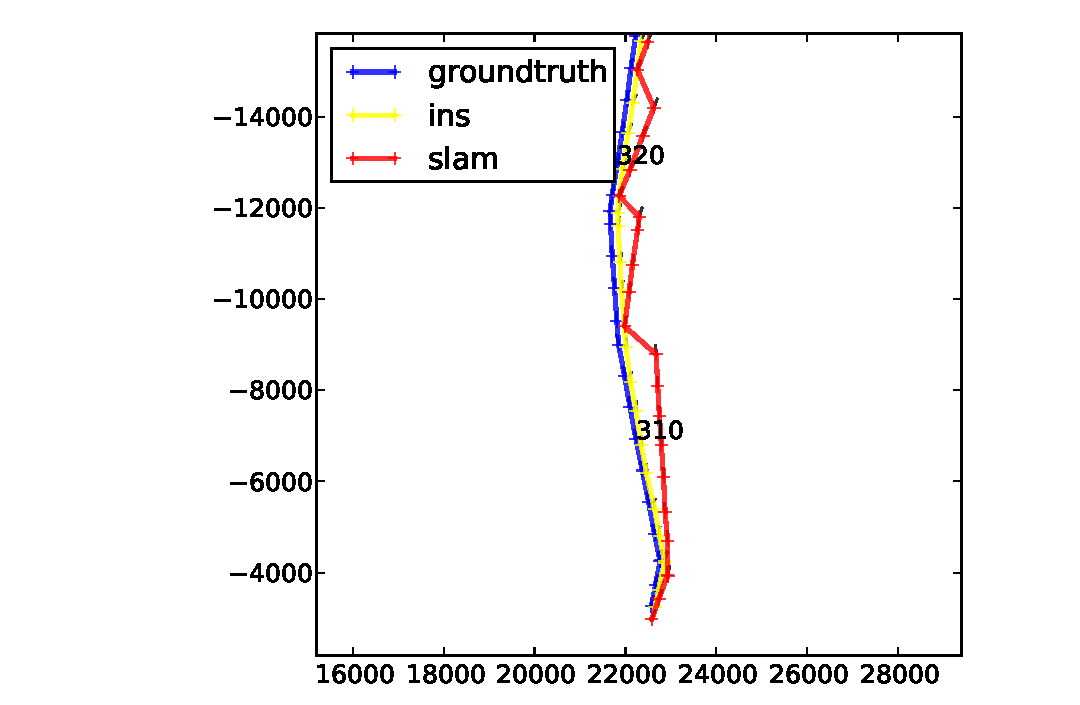
\includegraphics[width=0.7\textwidth]{images/experiment/map1/ins-problem.pdf}
  \caption{A small part of the path the robot moved in map 1. The wrong rotation estimate of the inertia sensor (yellow line) makes the slam-matcher (red line) think the robot moved in another direction than it did in reality (blue line). When the inertia sensor reading and SLAM result diverge too far, the SLAM location is reset to the inertia sensor estimate. This results in a jagged path estimate from the SLAM sensor.}
  \label{fig:map1-ins-problem}
\end{figure}

\subsection{Map 2}
Gotta make a second run.

\subsection{Map 3}
Gotta make a third run.

\section{Confidence measures}
The confidence measures of the first map are shown in figure~\ref{fig:map1-confidence-measures}.

\begin{figure}[ht]
  \centering
  \includegraphics[width=0.7\textwidth]{images/experiment/map1/confidence-measures.pdf}
  \caption{Confidence measures for map 1.}
  \label{fig:map1-ins-problem}
\end{figure}

\section{Map segments}

\section{Stitching}

\section{Results}